\documentclass[10pt]{beamer}
\usepackage[T1]{fontenc}
\usepackage{xeCJK}

\usetheme{Madrid}

\title{Hello World}
\subtitle[short subtitle]{long subtitle}
\author[dxy]{Xiangyun Ding}

\begin{document}

\frame{\titlepage}

\begin{frame}{A sample slide}
A displayed formula:
\[
  \int_{-\infty}^\infty e^{-x^2}\, dx = \sqrt{\pi}
\]
An itemized list:

\begin{itemize}
  \item itemized item 1,你好
  \item itemized item 2
\end{itemize}
\begin{enumerate}
  \item The first item
  \item The second item
\end{enumerate}

\end{frame}

\begin{frame}

\begin{theorem}{1.1}
  In a right triangle, \small{the square of hypotenuse equals
  the sum of squares of two} other sides.
\end{theorem}

\begin{block}{123}
  hello
\end{block}

\begin{description}
  \item[First Item] Description of first item
  \item[Second Item] Description of second item
\end{description}

\begin{columns}
  \column{.50\textwidth}
  First column text and/or code
  \column{.50\textwidth}
  Second column text and/or code
\end{columns}

\end{frame}

\begin{frame}{fff}
  \begin{table}
    \centering
    \caption{table decription}
    \label{t_sim}
    \begin{tabular}{|l|l|}
    \hline
    \textbf{Key} & \textbf{Value} \\
    \hline
    $x$ & description of x \\
    $y$ & description of y \\
    $y$ & description of z \\
    \hline
    \end{tabular}
    \end{table}

    \begin{table}[tb]
      \centering
      \caption{Caption here\label{tab:tablename}}
      \begin{tabular}{l|cc}
      \hline
      \textbf{column 1} & \textbf{column 2} & \textbf{column 3} \\ \hline
      Hello & Beamer & NAN \\ \hline
      $\alpha+\beta$ & $\gamma+\eta$ & 34\% \\ \hline
      \end{tabular}
      \end{table}

\end{frame}

\begin{frame}

  \begin{figure}[tb]
    \label{fig:figure1}
    \centering
    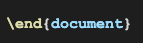
\includegraphics[width=0.5\textwidth]{t1.png}
    \caption{Caption here}
  \end{figure}

\end{frame}

\end{document}